% Document class and two-column conversion
\documentclass{report}
% dimensions of paper and relative text positioning
\usepackage[a4paper,top=2cm,bottom=2cm,left=2cm,right=2cm]{geometry}
% package for including URLs
\usepackage{url}
% Required for including images
\usepackage{graphicx}
\usepackage{float} % Required for specifying the exact location of a figure

% enable writing in greek
\usepackage[greek,english]{babel}
\usepackage[utf8]{inputenc}
%\usepackage[LGR]{fontenc}

\setlength{\parindent}{0pt} % Removes all indentation from paragraphs

% Start of the document
\begin{document}

% Set the language to greek
\selectlanguage{greek}

% Title page
\title{\Huge \bfseries Τεχνικές Βελτιστοποίησης \\ Δεύτερο Παραδοτέο} %\Huge and \bfseries are used to make the title bigger and bold
\author{Παπαδάκης Κωνσταντίνος Φώτιος\vspace{0.5cm} \\  ΑΕΜ:10371} % \vspace{0.5cm} is used to add some vertical space between the author and the AEM
\date{\today}
% prints the title, author and date on a separate page
\maketitle

% Table of contents page
\tableofcontents

% General introduction
\chapter{Εισαγωγή}
\section{Γενικά}
Η συνάρτηση πάνω στην οποία θα δουλέψουμε είναι η εξής:
$$f(x) = x^5 e^{-x^2-y^2}$$

Σχεδιάζουμε ένα \selectlanguage{english}Matlab script
\selectlanguage{greek}το οποίο παράγει τις πρώτες και δεύτερες μερικές παραγώγους της 
συνάρτησης $f(x,y)$:

\textbf{Πρώτη Μερική Παράγωγος}
\begin{itemize}
    \item Ως προς το $x$:
    $$\frac{\partial{z}}{\partial{x}} = 5x^4e^{-x^2-y^2} - 2x^6e^{-x^2-y^2}$$
    $$\frac{\partial{z}}{\partial{x}} = x^4(5-2x^2)e^{-x^2-y^2}$$
    \item Ως προς το $y$:
    $$\frac{\partial{z}}{\partial{y}} = -2x^{5}ye^{-x^2-y^2}$$
\end{itemize}

\textbf{Δεύτερη Μερική Παράγωγος}
\begin{itemize}
    \item Ως προς το $x$:
    $$\frac{\partial^2{z}}{\partial{x^2}} = 20x^{3}e^{-x^2-y^2}-22x^{5}e^{-x^2-y^2}+4x^{7}e^{-x^2-y^2}$$
    $$\frac{\partial^2{z}}{\partial{x^2}} = (20x^3 -22x^5 +4x^7)e^{-x^2-y^2}$$
    $$\frac{\partial^2{z}}{\partial{x^2}} = 2x^3(10-11x^2+2x^4)e^{-x^2-y^2}$$
    $$\frac{\partial^2{z}}{\partial{x^2}} = 2x^3(2x^2-1)(x^2-10)e^{-x^2-y^2}$$
    \item Ως προς το $y$:
    $$\frac{\partial^2{z}}{\partial{y^2}} = 4x^{5}y^{2}e^{-x^2-y^2} - 2x^{5}e^{-x^2-y^2}$$
    $$\frac{\partial^2{z}}{\partial{y^2}} = 2x^{5}(2y^2-1)e^{-x^2-y^2}$$
\end{itemize}
Πρόκειται να τις αξιοποιήσουμε κατά την εκτέλεση των αλγορίθμων για να μην υπολογίζουμε 
εντός αυτών τις τις παραγώγους αυτές που χρειάζονται συμβολική αναπαράσταση.
% Visualization of the function
\chapter{Θέμα 1}
\section{Εκφώνηση}
Σχεδιάστε την $f$ για να πάρετε μια γενική εικόνα της μορφής της.
\section{Λύση}
Χρησιμοποιώντας ένα απλό \selectlanguage{english}visualization script
\selectlanguage{greek}σε
\selectlanguage{english}Matlab
\selectlanguage{greek}εξάγουμε την παρακάτω εικόνα:
\begin{figure}[H]
    \centering
    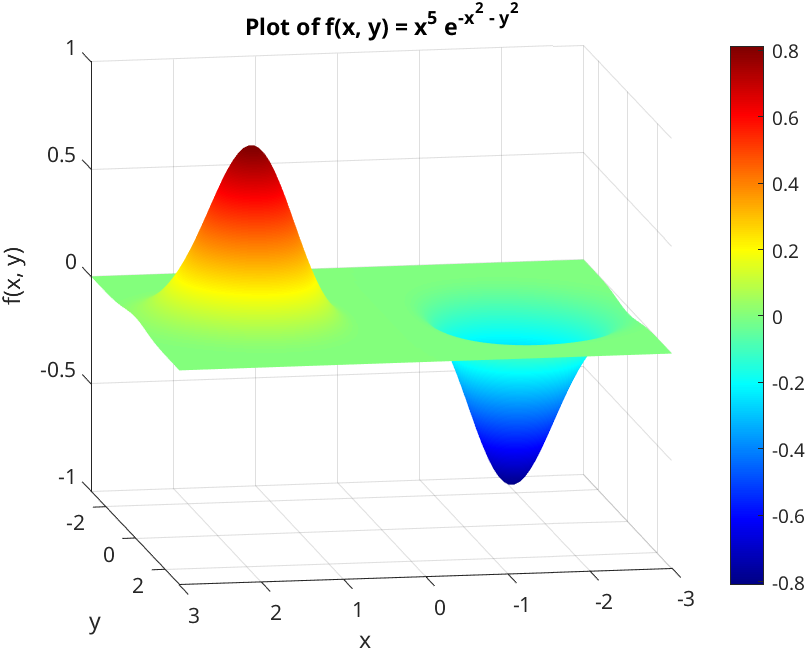
\includegraphics[width=0.5\textwidth]{media/visualization.png}
    \caption{Οπτικοποίηση της συνάρτησης $f(x,y)$}
\end{figure}

% Steepest Descent
\chapter{Θέμα 2}
\section{Εκφώνηση}
Ελαχιστοποιήστε την $f$ με την μέθοδο Μέγιστης Καθόδου, χρησιμοποιώντας ως αρχικά σημεία 
$(x, y)$ τα $i)$ $(0,0)$, $ii)$ $(-1,1)$, και $iii)$ $(1,-1)$. Το βήμα γ θα επιλεγεί: 
\begin{itemize}
    \item α) σταθερό (της επιλογής σας), 
    \item β) τέτοιο ώστε να ελαχιστοποιεί την $f(x + γd)$ και 
    \item γ) βάσει του κανόνα \selectlanguage{english}Armijo.
\end{itemize}
\selectlanguage{greek}
Σχολιάστε τις διαφορές στα αποτελέσματα, σε περίπτωση που προκαλούνται, λόγω της επιλογής του 
σημείου έναρξης $(x, y)$ του αλγορίθμου, καθώς επίσης και λόγω της επιλογής του βήματος γ.
δηγούμαστε πάντα σε σωστό αποτέλεσμα; Αν όχι, τι πιστεύετε ότι φταίει;

Σημείωση: Στην περίπτωση σταθερού βήματος δε χρειάζεται μαθηματική ανάλυση για τη συνθήκη σύγκλισης. 
Με βάση τη θεωρία εφαρμόστε τις τιμές απευθείας στο \selectlanguage{english}Matlab.
\selectlanguage{greek}
\section{Λύση}
\subsection{Περιγραφή Αλγορίθμου}
Στη μέθοδο της Μέγιστης Καθόδου κινούμαστε κόντρα στη φορά της μερικής παραγώγου της συνάρτησης
$f(x,y)$ έτσι ώστε να πλησιάσουμε πιο κοντά στο ελάχιστο της. Η εκτέλεση του κώδικα σταματάει 
όταν φτάσουμε τον μέγιστο αριθμό επαναλήψεων που ορίσαμε αυθαίρετα ή όταν η απόλυτη τιμή της 
παραγώγου της συνάρτησης γίνει μικρότερη από μια σταθερά ανοχής που μας επιτρέπει να πλησιάσουμε 
αρκετά στο σημείο ελάχιστου χωρίς να παρατείνουμε την εκτέλεση του αλγορίθμου παραπάνω από όσο
είναι αναγκαίο.

\subsection{Αποτελέσματα}
Τα σημεία εκκίνησης που μας δόθηκαν είναι τα εξής:
\begin{itemize}
    \item \([0,0]\): Είναι ένα σημείο στο οποίο η παράγωγος είναι εξαρχής πολύ κοντά στο μηδέν και άρα 
    ο αλγόριθμος σταματάει αμέσως, ακόμα και για πολύ μικρή σταθερά ανοχής.
    \item \([-1,1]\): Βρισκόμαστε σε σημείο όπου η μερική παράγωγος μπορεί να ακολουθήσει πορεία προς το
    ελάχιστο. Αυτό φαίνεται πρακτικά και στα αποτελέσματα.
    \item \([1,-1]\): Βρισκόμαστε σε μια περιοχή όπου ξεκινάει η ανάβαση προς το ολικό μέγιστο. Επομένως
    ο αλγόριθμος θα αποκλίνει από το σημείο εκείνο και θα ανατρέξει το ελάχιστο προς την αντίθετη φορά
    όπου και θα τερματίσει σε ένα σημείο όπου η παράγωγος είναι πολύ κοντά στο μηδέν.
\end{itemize}
Το βήμα με το οποίο μετακινούμαστε στον χώρο το ορίζουμε με έναν από ο τους εξής τρόπους:
\begin{itemize}
    \item Σταθερό βήμα\\
    \textbf{Μεθοδολογία:} Για βήμα $0.001$ και ανοχή $10^{-4}$ παρατηρούμε ότι ο αλγόριθμος συγκλίνει
    μετά από:
    \begin{itemize}
        \item \([0,0]\): 0 επαναλήψεις, όπου $f(0,0) = 0$
        \item \([-1,1]\): 6632 επαναλήψεις, όπου $f(-1.5811, 0.0001) = -0.811174$
        \item \([1,-1]\): 343491 επαναλήψεις, όπου $f(0.1545, -1.2849) =  0.000016$
    \end{itemize}
    
    \item Βήμα που ελαχιστοποιεί την $f(x + γd)$\\
    \textbf{Μεθοδολογία:} Για βήμα που ελαχιστοποιεί την $f(x_k + gamma_k * d_k)$ και ανοχή $10^{-4}$
    ο αλγόριθμος συγκλίνει μετά από:
    \begin{itemize}
        \item \([0,0]\): 0 επαναλήψεις, όπου $f(0,0) = 0$
        \item \([-1,1]\): 9 επαναλήψεις, όπου $f(-1.5811, 0.0000) = -0.811174$
        \item \([1,-1]\): 359 επαναλήψεις, όπου $f(0.1074, -1.3718) = 0.000002$
    \end{itemize}
    \item Βήμα βάσει του κανόνα \selectlanguage{english}Armijo\selectlanguage{greek}\\
    \textbf{Μεθοδολογία:} Για βήμα όπου ισχύει\\
    $$γ_k = s \beta^m_k$$ και 
    $$f(x_k)-f(x_k+1)>=\alpha \beta^{m_k} s d_k^T \nabla f(x_k)$$
    ο αλγόριθμος συγκλίνει μετά από:
    \begin{itemize}
        \item \([0,0]\): 0 επαναλήψεις, όπου $f(0,0) = 0$
        \item \([-1,1]\): 20 επαναλήψεις, όπου $f(-1.5812, 0.0000) = -0.811174$
        \item \([1,-1]\): 359 επαναλήψεις, όπου $f(0.1074, -1.3718) = 0.000002$
    \end{itemize}
\end{itemize}


% Newton
\chapter{Θέμα 3}
\section{Εκφώνηση}
Επαναλάβετε τα ερωτήματα του Θέματος 2 χρησιμοποιώντας την μέθοδο 
\selectlanguage{english}Newton.
\selectlanguage{greek}
\section{Λύση}
\subsection{Περιγραφή Αλγορίθμου}
Ο Αλγόριθμος του Νεύτωνα βασίζεται στον υπολογισμό του Εσσιανού πίνακα με σκοπό την γρηγορότερη
σύγκλιση στο ελάχιστο. Ο αλγόριθμος αυτός όπως και ο επόμενος στη σειρά αφορμόνται από το σταθερό,
σε κάθε επανάληψη, βήμα το οποίο δεν προσαρμόζεται βάσει της περιβάλλουσας γεωμετρίας. Στην περίπτωση
του αλγορίθμου του Νεύτωνα υπολογίζουμε την κατεύθυνση αναζήτησης $d_k$ με τον τύπο: 
$$d_k = -H_k^{-1} \nabla f(x_k)$$
Έπειτα υπολογίζουμε το επόμενο σημείο $x_{k+1}$ με τον τύπο:
$$x_{k+1} = x_k + \gamma_k d_k$$
και επαναλαμβάνουμε την παραπάνω διαδικασία ωσότου η μερική παράγωγος της συνάρτησης $f(x,y)$
γίνει μικρότερη από τη σταθερά ανοχής που αναφέραμε και στον προηγούμενο αλγόριθμο. 

\subsection{Αποτελέσματα}
Τα σημεία εκκίνησης είναι ίδια με το Θέμα 2.\\
Το βήμα με το οποίο μετακινούμαστε στον χώρο το ορίζουμε με έναν από ο τους εξής τρόπους:
\begin{itemize}
    \item Σταθερό βήμα\\
    \textbf{Μεθοδολογία:} Για βήμα $0.001$ και ανοχή $10^{-4}$ παρατηρούμε ότι ο αλγόριθμος συγκλίνει
    μετά από:
    \begin{itemize}
        \item \([0,0]\): 0 επαναλήψεις, όπου $f(0,0) = 0$
        \item \([-1,1]\): 9782 επαναλήψεις, όπου $f(-0.1318, 1.6409) = -0.000003$
        \item \([1,-1]\): 9782 επαναλήψεις, όπου $f(1.6409, -0.1318) = 0.000003$
    \end{itemize}
    
    \item Βήμα που ελαχιστοποιεί την $f(x + γd)$\\
    \textbf{Μεθοδολογία:} Για βήμα που ελαχιστοποιεί την $f(x_k + gamma_k * d_k)$ και ανοχή $10^{-4}$
    ο αλγόριθμος συγκλίνει μετά από:
    \begin{itemize}
        \item \([0,0]\): 0 επαναλήψεις, όπου $f(0,0) = 0$
        \item \([-1,1]\): 147976 επαναλήψεις, όπου $f(-0.1318, 1.6409) = -0.000003$
        \item \([1,-1]\): 9 επαναλήψεις, όπου $f(0.1251, -1.6063) = 0.000002$
    \end{itemize}
    \item Βήμα βάσει του κανόνα \selectlanguage{english}Armijo\selectlanguage{greek}\\
    \textbf{Μεθοδολογία:} Για βήμα όπου ισχύει\\
    $$γ_k = s \beta^m_k$$ και 
    $$f(x_k)-f(x_k+1)>=\alpha \beta^{m_k} s d_k^T \nabla f(x_k)$$
    ο αλγόριθμος συγκλίνει μετά από:
    \begin{itemize}
        \item \([0,0]\): 0 επαναλήψεις, όπου $f(0,0) = 0$
        \item \([-1,1]\): >300000 επαναλήψεις, όπου $f(-1.0000, 1.0000) = -0.135335$
        \item \([1,-1]\): 9 επαναλήψεις, όπου $f(0.1251, -1.6063) = 0.000002$
    \end{itemize}
\end{itemize}


% Levenberg Marquardt
\chapter{Θέμα 4}
\section{Εκφώνηση}
Επαναλάβετε τα ερωτήματα του Θέματος 2 χρησιμοποιώντας την μέθοδο 
\selectlanguage{english}Levenberg-Marquardt.
\selectlanguage{greek} 
\section{Λύση}
\subsection{Περιγραφή Αλγορίθμου}
Ο τελευταίος αλγόριθμος που θα εξετάσουμε είναι ο αλγόριθμος \selectlanguage{english}
Levenberg-Marquardt. \selectlanguage{greek}Αποτελεί προέκταση του αλγορίθμου του Νεύτωνα και
του αλγορίθμου της Μέγιστης Καθόδου. Αρχικά υπολογίζουμε το $μ_k$ τέτοιο ώστε:
$$(H_k + μ_kI)d_k = -\nabla f(x_k)$$
Στη συνέχεια υπολογίζουμε το $\gamma_k$ ώστε να ικανοποιούνται οι σχέσεις:
$$d_k^T\nabla f(x_k) < 0$$
$$d_k^T\nabla f(x_k+1) > \beta d_k^T\nabla f(x_k)$$
Τέλος υπολογίζουμε το επόμενο σημείο $x_{k+1}$ με τον τύπο:
$$x_{k+1} = x_k + \gamma_k d_k$$

\subsection{Αποτελέσματα}
Τα σημεία εκκίνησης είναι ίδια με το Θέμα 2.\\
Το βήμα με το οποίο μετακινούμαστε στον χώρο το ορίζουμε με έναν από ο τους εξής τρόπους:
\begin{itemize}
    \item Σταθερό βήμα\\
    \textbf{Μεθοδολογία:} Για βήμα $0.001$ και ανοχή $10^{-4}$ παρατηρούμε ότι ο αλγόριθμος συγκλίνει
    μετά από:
    \begin{itemize}
        \item \([0,0]\): 0 επαναλήψεις, όπου $f(0,0) = 0$
        \item \([-1,1]\): 21222 επαναλήψεις, όπου $f(0.6265, -49.7396) = 0$
        \item \([1,-1]\): 9782 επαναλήψεις, όπου $f(0.1318, -1.6409) = 0.000003$
    \end{itemize}
    
    \item Βήμα που ελαχιστοποιεί την $f(x + γd)$\\
    \textbf{Μεθοδολογία:} Για βήμα που ελαχιστοποιεί την $f(x_k + gamma_k * d_k)$ και ανοχή $10^{-4}$
    ο αλγόριθμος συγκλίνει μετά από:
    \begin{itemize}
        \item \([0,0]\): 0 επαναλήψεις, όπου $f(0,0) = 0$
        \item \([-1,1]\): 101 επαναλήψεις, όπου $f(-1.5811, 0.0001) = -0.811174$
        \item \([1,-1]\): 9 επαναλήψεις, όπου $f(0.1251, -1.6063) = 0.000002$
    \end{itemize}
    \item Βήμα βάσει του κανόνα \selectlanguage{english}Armijo\selectlanguage{greek}\\
    \textbf{Μεθοδολογία:} Για βήμα όπου ισχύει\\
    $$γ_k = s \beta^m_k$$ και 
    $$f(x_k)-f(x_k+1)>=\alpha \beta^{m_k} s d_k^T \nabla f(x_k)$$
    ο αλγόριθμος συγκλίνει μετά από:
    \begin{itemize}
        \item \([0,0]\): 0 επαναλήψεις, όπου $f(0,0) = 0$
        \item \([-1,1]\): 119 επαναλήψεις, όπου $f(-1.5811, 0.0001) = -0.811174$
        \item \([1,-1]\): 9 επαναλήψεις, όπου $f(0.1251, -1.6063) = 0.000002$
    \end{itemize}
\end{itemize}


% Comparison
\chapter{Ανάλυση αποτελεσμάτων}
\section{Γραφήματα}
Παρουσιάζουμε τις γραφικές παραστάσεις των τιμών της συνάρτησης $f(x,y)$ ως προς τις επαναλήψεις. 
Σε αυτές θα περιορίσουμε τον αριθμό των μέγιστων επαναλήψεων έτσι ώστε να διατηρήσουμε την περισσότερη
πληροφορία που μπορεί να μας δώσει το εκάστοτε γράφημα.\\ 
Για την μέθοδο μέγιστης καθόδου έχουμε:
\begin{itemize}
    \item Στο [0,0] το γράφημα είναι σταθερά στο 0.
    \item Στο [-1,1]:
    \begin{figure}[H]
        \centering
        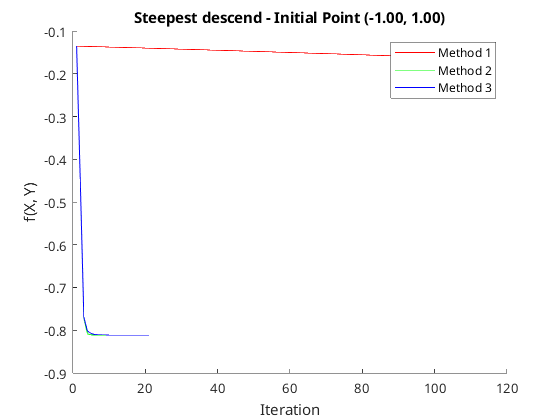
\includegraphics[width=0.5\textwidth]{media/steep-11.png}
        \caption{Μέγιστη Κάθοδος [-1,1]}
    \end{figure}
    \item Στο [1,-1]:
    \begin{figure}[H]
        \centering
        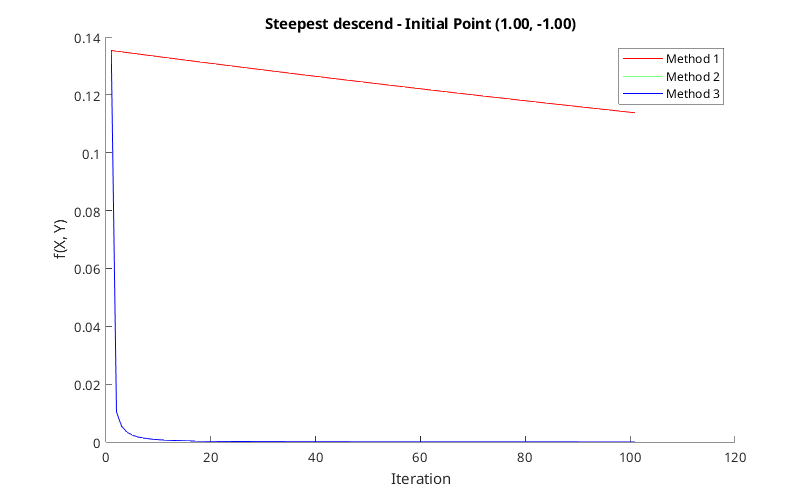
\includegraphics[width=0.5\textwidth]{media/steep1-1.png}
        \caption{Μέγιστη Κάθοδος [1,-1]}
    \end{figure}
\end{itemize}

Για την μέθοδο \selectlanguage{english}Newton\selectlanguage{greek} έχουμε:
\begin{itemize}
    \item Στο [0,0] το γράφημα είναι σταθερά στο 0.
    \item Στο [-1,1]:
    \begin{figure}[H]
        \centering
        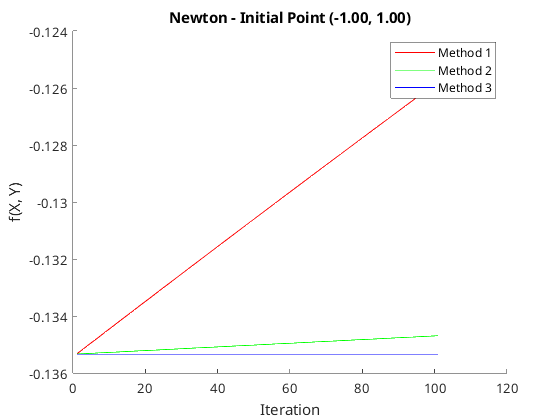
\includegraphics[width=0.5\textwidth]{media/newton-11.png}
        \caption{\selectlanguage{english}Newton\selectlanguage{greek} [-1,1]}
    \end{figure}
    \item Στο [1,-1]:
    \begin{figure}[H]
        \centering
        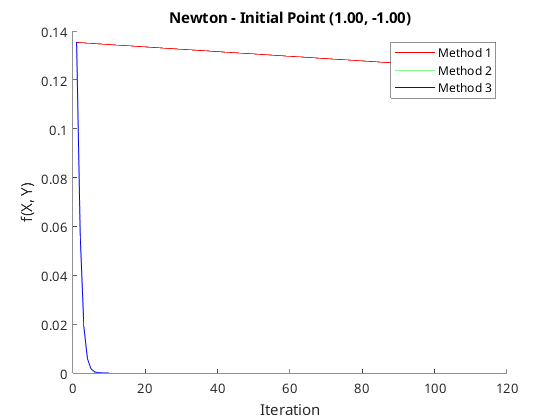
\includegraphics[width=0.5\textwidth]{media/newton1-1.png}
        \caption{\selectlanguage{english}Newton\selectlanguage{greek} [1,-1]}
    \end{figure}
\end{itemize}

Για την μέθοδο \selectlanguage{english}Levenberg-Marquardt\selectlanguage{greek} έχουμε:
\begin{itemize}
    \item Στο [0,0] το γράφημα είναι σταθερά στο 0.
    \item Στο [-1,1]:
    \begin{figure}[H]
        \centering
        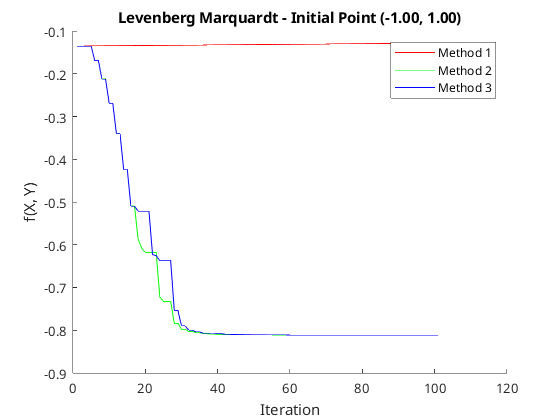
\includegraphics[width=0.5\textwidth]{media/leven-11.png}
        \caption{\selectlanguage{english}Levenberg-Marquardt\selectlanguage{greek} [1,-1]}
    \end{figure}
    \item Στο [1,-1]:
    \begin{figure}[H]
        \centering
        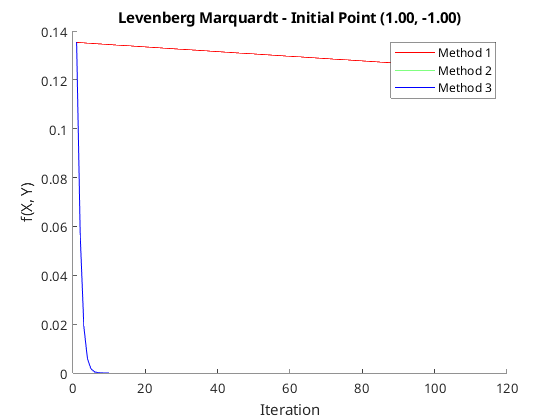
\includegraphics[width=0.5\textwidth]{media/leven1-1.png}
        \caption{\selectlanguage{english}Levenberg-Marquardt\selectlanguage{greek} [1,-1]}
    \end{figure}
\end{itemize}

\section{Σχόλια}
Κατά κανόνα η μέθοδος του σταθερού βήματος ήταν η πιο αργή σε όλα τα τεστ που διενεργήθηκαν.
Η μεταβλητότητα των μεθόδων 2 και 3 αυξάνουν την ταχύτητα δραματικά. 

\subsection{Αλγόριθμος Μέγιστης Καθόδου}
Εδώ βλέπουμε τα αναμενόμενα αποτελέσματα εκτός από την περίπτωση του \([-1,1]\) όπου το σταθερό
βήμα δεν μπόρεσε να μας οδηγήσει στη σωστή απάντηση. Το $y$ καταλήγει να βηματίζει περισσότερο 
από ότι θα έπρεπε και χάνει την καμπύλη μέσω της οποίας θα μπορούσε να οδηγηθεί στο ελάχιστο και 
ψάχνει κάποια άλλη πορεία με βάση τα καινούρια της δεδομένα στο νέο σημείο στο οποίο μόλις έφτασε.

\subsection{Αλγόριθμος \selectlanguage{english}Newton\selectlanguage{greek}}
Ο αλγόριθμος του Νεύτωνα δεν μας οδήγησε στο ελάχιστο επειδή ο Εσσιανός πίνακας δεν ήταν θετικός
στην κατεύθυνση του υπολογισμού.

\subsection{Αλγόριθμος \selectlanguage{english}Levenberg-Marquardt\selectlanguage{greek}}
Ο αλγόριθμος των \selectlanguage{english}Levenberg-Marquardt\selectlanguage{greek} μας οδήγησε στο ελάχιστο
όμως πλήττεται από το ίδιο πρόβλημα με τον αλγόριθμο της Μέγιστης Καθόδου όπου με σταθερό βήμα μειώνεται 
πολύ το $y$ και φεύγει από την περιοχή του ελάχιστου.


% Bibliography
\nocite{*} % Include all references in the bibliography, even if they are not cited in the report
\bibliographystyle{plain}
\bibliography{references/references} % We have to include the references somewhere in the report for them to show here if we don't use (\nocite{*})
\addcontentsline{toc}{chapter}{\bibname} % Add the bibliography to the table of contents

% End of the document
\end{document}